\documentclass[preview]{standalone}
\usepackage{tikz}
\begin{document}
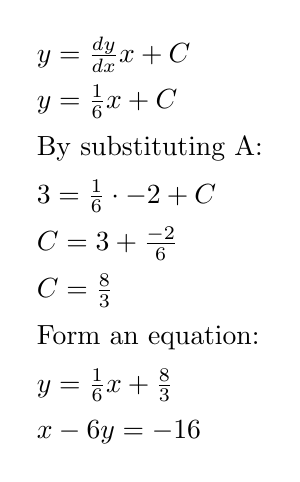
\begin{tikzpicture}[domain=0:2]
\node[right] at (0,0){$y = \frac{dy}{dx}x + C$};
\node[right] at (0, -0.6){$y = \frac{1}{6}x + C$};
\node[right] at (0, -1.2){By substituting A:};
\node[right] at (0, -1.8){$3 = \frac{1}{6}\cdot-2 + C$};
\node[right] at (0, -2.4){$C = 3 + \frac{-2}{6}$};
\node[right] at (0, -3){$C = \frac{8}{3}$};
\node[right] at (0, -3.6){Form an equation:};
\node[right] at (0, -4.2){$y = \frac{1}{6}x + \frac{8}{3}$};
\node[right] at (0, -4.8){$x - 6y = -16$};
\end{tikzpicture}
\end{document}